\newpage
\subsection{Funktionsgleichung bestimmen}

Es gibt zwei Arten der Bestimmung der Funktionsgleichung:\\

\hfill \break
\fboxrule=0.8pt \fcolorbox{black}{lightgray}{%
    \begin{tabular}[t]{@{}l@{}}
        $A(1/8)$  \\
        $B(-4/3)$ \\
        \hline
        $y=kx+d$
    \end{tabular}}\\

\hfill \break
1.Graphisch:\\
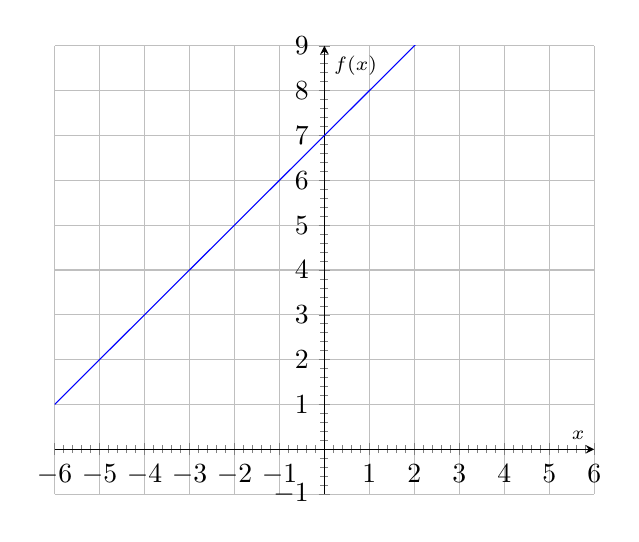
\begin{tikzpicture}[scale=1.0]
    \begin{axis}%
        [
            grid=major,
            xtick={-7,-6,...,7},
            minor x tick num=4, % 4 minor ticks => 5 subintervals
            xmin=-6,
            xmax=6,
            xlabel={\scriptsize $x$},
            axis x line=middle,
            ytick={-5,-4,...,9},
            minor y tick num=4,  % 4 minor ticks => 5 subintervals
            ymin=-1,
            ymax=9,
            ylabel={\scriptsize $f(x)$},
            axis y line=middle,
            no markers,
            samples=100,
            domain=-6:6,
        ]
        \addplot[blue] (x,{x+7});
    \end{axis}
\end{tikzpicture}

\hfill \break
\fboxrule=0.8pt \fcolorbox{black}{lightgray}{%
    \begin{tabular}[t]{@{}l@{}}
            $d=7$ \\
            $k=1$ \\
            \hline
            $y=kx+d$
        \end{tabular}}\\

\hfill \break
2.Rechnerisch:\\
\fboxrule=0.8pt \fcolorbox{black}{lightgray}{%
    \begin{tabular}[t]{@{}l@{}}
            (1):$8=1k+d$                                            \\
            (2):$\textcolor{blue}{3=-4k+d}$                         \\
            (1):$d=-k+8$                                            \\
            $3=-4k-k+8$ / ermittelt durch das Eliminationsverfahren \\
            $k=\textcolor{red}{1}$                                  \\
            \\
            $\textcolor{blue}{3=-4*\textcolor{red}{1}+d}$           \\
            $d=7$                                                   \\
        \end{tabular}}\\